\documentclass{standalone}
\usepackage{tikz}
\usetikzlibrary{patterns}
\usetikzlibrary{positioning}
\usetikzlibrary{patterns, positioning}
\usetikzlibrary{shapes.misc}
\usepackage[outline]{contour}
\contourlength{1.5pt} 
\usetikzlibrary{calc}
        \usepackage{relsize}
        \tikzset{fontscale/.style = {font=\relsize{#1}}}

\begin{document}
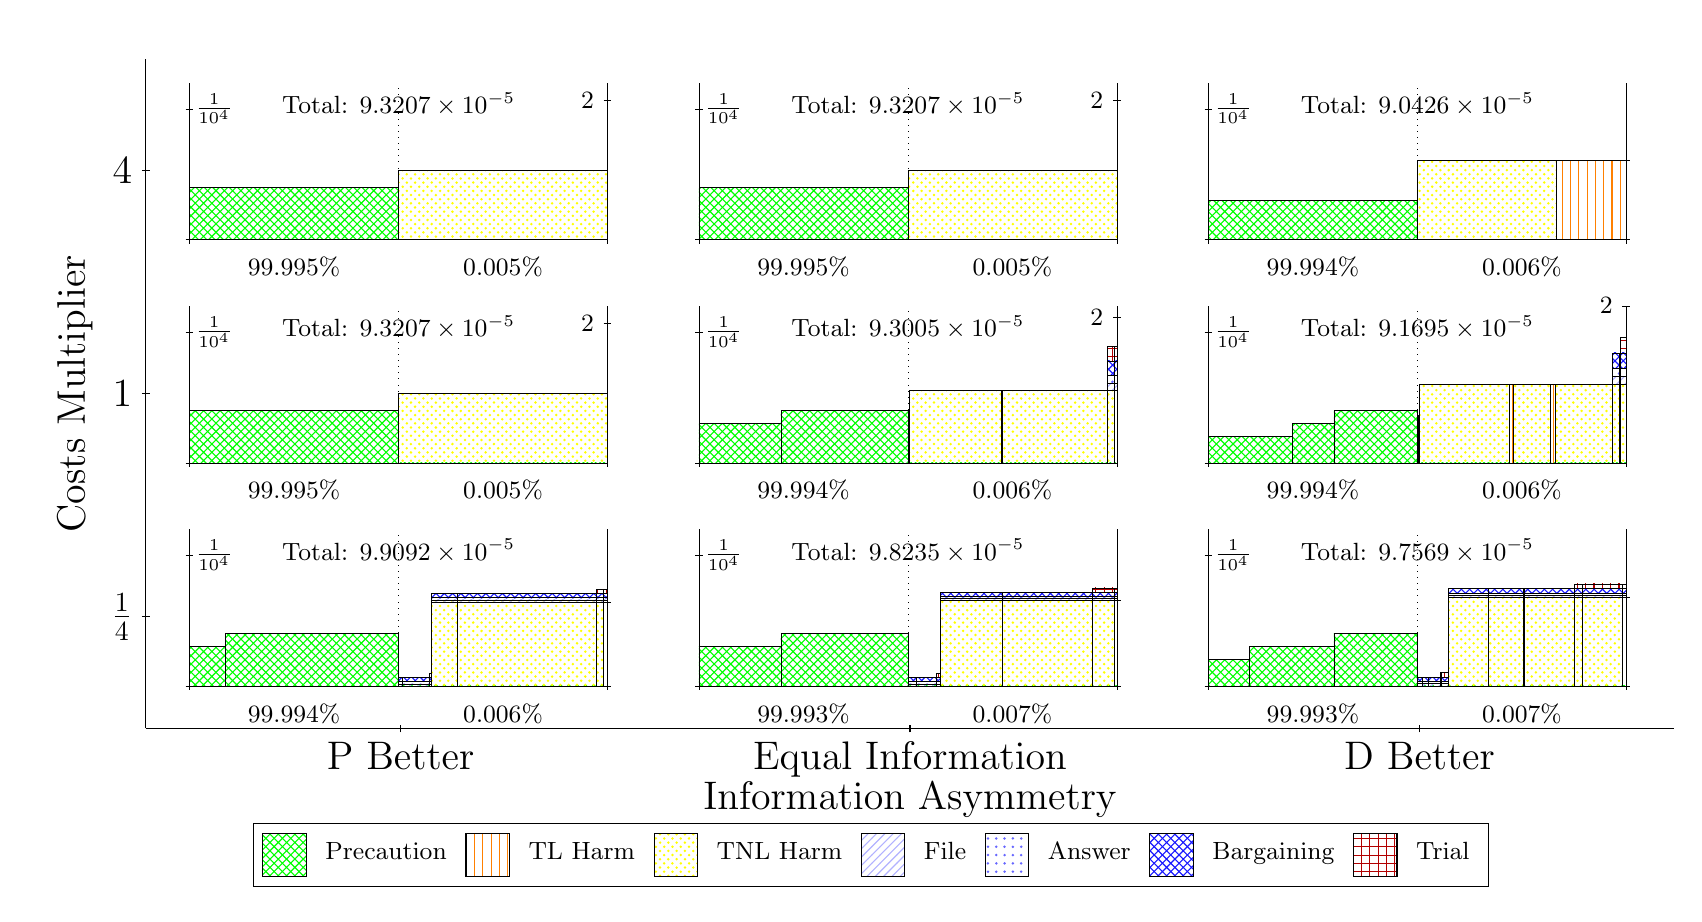
\begin{tikzpicture}
\clip(-0.5,-1.1) rectangle +(20.91,11);
\draw[black] (1,1) -- (1,9.5);
\node[rotate=90, fontscale=2, anchor=center] at (0.1, 5.25) {Costs Multiplier};
\draw[black] (0.95,2.4167) -- (1.05,2.4167);
\node[fontscale=2, anchor=east] at (0.95, 2.4167) {$\frac{1}{4}$};
\draw[black] (0.95,5.25) -- (1.05,5.25);
\node[fontscale=2, anchor=east] at (0.95, 5.25) {1};
\draw[black] (0.95,8.0833) -- (1.05,8.0833);
\node[fontscale=2, anchor=east] at (0.95, 8.0833) {4};

\draw[black] (1,1) -- (20.41,1);
\node[fontscale=2, anchor=center] at (10.705, 0.1) {Information Asymmetry};
\draw[black] (4.235,0.95) -- (4.235,1.05);
\node[fontscale=2, anchor=north] at (4.235, 0.95) {P Better};
\draw[black] (10.705,0.95) -- (10.705,1.05);
\node[fontscale=2, anchor=north] at (10.705, 0.95) {Equal Information};
\draw[black] (17.175,0.95) -- (17.175,1.05);
\node[fontscale=2, anchor=north] at (17.175, 0.95) {D Better};


\draw[pattern=crosshatch, pattern color=green,draw=black,very thin] (1.5556,1.54) rectangle (2.0149,2.0384);
\draw[pattern=crosshatch, pattern color=green,draw=black,very thin] (2.0149,1.54) rectangle (4.21,2.2045);
\draw[pattern=crosshatch, pattern color=green,draw=black,very thin] (4.21,1.54) rectangle (4.2564,1.54);
\draw[pattern=north east lines, pattern color=blue!30,draw=black,very thin] (4.21,1.54) rectangle (4.2564,1.5667);
\draw[pattern=dots,  pattern color=blue!60,draw=black,very thin] (4.21,1.5667) rectangle (4.2564,1.5934);
\draw[pattern=crosshatch,      pattern color=blue!90,draw=black,very thin] (4.21,1.5934) rectangle (4.2564,1.6467);
\draw[pattern=crosshatch, pattern color=green,draw=black,very thin] (4.2564,1.54) rectangle (4.5983,1.54);
\draw[pattern=north east lines, pattern color=blue!30,draw=black,very thin] (4.2564,1.54) rectangle (4.5983,1.5667);
\draw[pattern=dots,  pattern color=blue!60,draw=black,very thin] (4.2564,1.5667) rectangle (4.5983,1.5934);
\draw[pattern=crosshatch,      pattern color=blue!90,draw=black,very thin] (4.2564,1.5934) rectangle (4.5983,1.6467);
\draw[pattern=crosshatch, pattern color=green,draw=black,very thin] (4.5983,1.54) rectangle (4.6234,1.54);
\draw[pattern=north east lines, pattern color=blue!30,draw=black,very thin] (4.5983,1.54) rectangle (4.6234,1.5667);
\draw[pattern=dots,  pattern color=blue!60,draw=black,very thin] (4.5983,1.5667) rectangle (4.6234,1.5934);
\draw[pattern=crosshatch,      pattern color=blue!90,draw=black,very thin] (4.5983,1.5934) rectangle (4.6234,1.6467);
\draw[pattern=grid,            pattern color=red!70!black,draw=black,very thin] (4.5983,1.6467) rectangle (4.6234,1.7);
\draw[pattern=crosshatch, pattern color=green,draw=black,very thin] (4.6234,1.54) rectangle (4.9562,1.54);
\draw[pattern=crosshatch dots, pattern color=yellow,draw=black,very thin] (4.6234,1.54) rectangle (4.9562,2.6066);
\draw[pattern=north east lines, pattern color=blue!30,draw=black,very thin] (4.6234,2.6066) rectangle (4.9562,2.6333);
\draw[pattern=dots,  pattern color=blue!60,draw=black,very thin] (4.6234,2.6333) rectangle (4.9562,2.66);
\draw[pattern=crosshatch,      pattern color=blue!90,draw=black,very thin] (4.6234,2.66) rectangle (4.9562,2.7133);
\draw[pattern=crosshatch, pattern color=green,draw=black,very thin] (4.9562,1.54) rectangle (6.7215,1.54);
\draw[pattern=crosshatch dots, pattern color=yellow,draw=black,very thin] (4.9562,1.54) rectangle (6.7215,2.6067);
\draw[pattern=north east lines, pattern color=blue!30,draw=black,very thin] (4.9562,2.6067) rectangle (6.7215,2.6333);
\draw[pattern=dots,  pattern color=blue!60,draw=black,very thin] (4.9562,2.6333) rectangle (6.7215,2.66);
\draw[pattern=crosshatch,      pattern color=blue!90,draw=black,very thin] (4.9562,2.66) rectangle (6.7215,2.7133);
\draw[pattern=crosshatch, pattern color=green,draw=black,very thin] (6.7215,1.54) rectangle (6.8057,1.54);
\draw[pattern=crosshatch dots, pattern color=yellow,draw=black,very thin] (6.7215,1.54) rectangle (6.8057,2.6066);
\draw[pattern=north east lines, pattern color=blue!30,draw=black,very thin] (6.7215,2.6066) rectangle (6.8057,2.6333);
\draw[pattern=dots,  pattern color=blue!60,draw=black,very thin] (6.7215,2.6333) rectangle (6.8057,2.66);
\draw[pattern=crosshatch,      pattern color=blue!90,draw=black,very thin] (6.7215,2.66) rectangle (6.8057,2.7133);
\draw[pattern=grid,            pattern color=red!70!black,draw=black,very thin] (6.7215,2.7133) rectangle (6.8057,2.7666);
\draw[pattern=crosshatch, pattern color=green,draw=black,very thin] (6.8057,1.54) rectangle (6.8644,1.54);
\draw[pattern=vertical lines, pattern color=orange,draw=black,very thin] (6.8057,1.54) rectangle (6.8644,2.6066);
\draw[pattern=north east lines, pattern color=blue!30,draw=black,very thin] (6.8057,2.6066) rectangle (6.8644,2.6333);
\draw[pattern=dots,  pattern color=blue!60,draw=black,very thin] (6.8057,2.6333) rectangle (6.8644,2.66);
\draw[pattern=crosshatch,      pattern color=blue!90,draw=black,very thin] (6.8057,2.66) rectangle (6.8644,2.7133);
\draw[pattern=grid,            pattern color=red!70!black,draw=black,very thin] (6.8057,2.7133) rectangle (6.8644,2.7666);
\node[font=\small,text=black,anchor=north] at (4.21, 3.5333) {Total: $9.9092\times 10^{-5}$};
\draw[black,very thin] (1.5556,1.54) -- (1.5556,3.5333);
\draw[black,very thin] (1.5056,1.54) -- (1.6056,1.54);
\node[font=\small,text=black, anchor=west] at (1.5056, 1.54) {};
\draw[black,very thin] (1.5056,3.2013) -- (1.6056,3.2013);
\node[font=\small,text=black, anchor=west] at (1.5056, 3.2013) {$\frac{1}{10^{4}}$};

\draw[black,dotted,very thin] (4.21,1.5998) -- (4.21,3.4735);
\draw[black,very thin] (6.8644,1.54) -- (6.8644,3.5333);
\draw[black,very thin] (6.8144,1.54) -- (6.9144,1.54);
\node[font=\small,text=black, anchor=east] at (6.8144, 1.54) {\contour{white}{}};
\draw[black,very thin] (6.8144,2.6066) -- (6.9144,2.6066);
\node[font=\small,text=black, anchor=east] at (6.8144, 2.6066) {\contour{white}{}};

\draw[black,very thin] (1.5556,1.54) -- (6.8644,1.54);
\draw[black,very thin] (1.5556,1.49) -- (1.5556,1.59);
\node[font=\small,text=black, anchor=north] at (1.5556, 1.49) {};
\draw[black,very thin] (6.8644,1.49) -- (6.8644,1.59);
\node[font=\small,text=black, anchor=north] at (6.8644, 1.49) {};

\node[font=\small,text=black,anchor=south] at (2.8828, 0.94) {99.994\%};
\node[font=\small,text=black,anchor=south] at (5.5372, 0.94) {0.006\%};

\draw[pattern=crosshatch, pattern color=green,draw=black,very thin] (8.0256,1.54) rectangle (9.0658,2.0384);
\draw[pattern=crosshatch, pattern color=green,draw=black,very thin] (9.0658,1.54) rectangle (10.68,2.2045);
\draw[pattern=crosshatch, pattern color=green,draw=black,very thin] (10.68,1.54) rectangle (10.791,1.54);
\draw[pattern=north east lines, pattern color=blue!30,draw=black,very thin] (10.68,1.54) rectangle (10.791,1.5671);
\draw[pattern=dots,  pattern color=blue!60,draw=black,very thin] (10.68,1.5671) rectangle (10.791,1.5942);
\draw[pattern=crosshatch,      pattern color=blue!90,draw=black,very thin] (10.68,1.5942) rectangle (10.791,1.6483);
\draw[pattern=crosshatch, pattern color=green,draw=black,very thin] (10.791,1.54) rectangle (11.039,1.54);
\draw[pattern=north east lines, pattern color=blue!30,draw=black,very thin] (10.791,1.54) rectangle (11.039,1.5671);
\draw[pattern=dots,  pattern color=blue!60,draw=black,very thin] (10.791,1.5671) rectangle (11.039,1.5942);
\draw[pattern=crosshatch,      pattern color=blue!90,draw=black,very thin] (10.791,1.5942) rectangle (11.039,1.6484);
\draw[pattern=crosshatch, pattern color=green,draw=black,very thin] (11.039,1.54) rectangle (11.087,1.54);
\draw[pattern=north east lines, pattern color=blue!30,draw=black,very thin] (11.039,1.54) rectangle (11.087,1.5671);
\draw[pattern=dots,  pattern color=blue!60,draw=black,very thin] (11.039,1.5671) rectangle (11.087,1.5942);
\draw[pattern=crosshatch,      pattern color=blue!90,draw=black,very thin] (11.039,1.5942) rectangle (11.087,1.6483);
\draw[pattern=grid,            pattern color=red!70!black,draw=black,very thin] (11.039,1.6483) rectangle (11.087,1.7025);
\draw[pattern=crosshatch, pattern color=green,draw=black,very thin] (11.087,1.54) rectangle (11.879,1.54);
\draw[pattern=crosshatch dots, pattern color=yellow,draw=black,very thin] (11.087,1.54) rectangle (11.879,2.6232);
\draw[pattern=north east lines, pattern color=blue!30,draw=black,very thin] (11.087,2.6232) rectangle (11.879,2.6502);
\draw[pattern=dots,  pattern color=blue!60,draw=black,very thin] (11.087,2.6502) rectangle (11.879,2.6773);
\draw[pattern=crosshatch,      pattern color=blue!90,draw=black,very thin] (11.087,2.6773) rectangle (11.879,2.7315);
\draw[pattern=crosshatch, pattern color=green,draw=black,very thin] (11.879,1.54) rectangle (11.881,1.54);
\draw[pattern=vertical lines, pattern color=orange,draw=black,very thin] (11.879,1.54) rectangle (11.881,2.6232);
\draw[pattern=north east lines, pattern color=blue!30,draw=black,very thin] (11.879,2.6232) rectangle (11.881,2.6502);
\draw[pattern=dots,  pattern color=blue!60,draw=black,very thin] (11.879,2.6502) rectangle (11.881,2.6773);
\draw[pattern=crosshatch,      pattern color=blue!90,draw=black,very thin] (11.879,2.6773) rectangle (11.881,2.7315);
\draw[pattern=crosshatch, pattern color=green,draw=black,very thin] (11.881,1.54) rectangle (13.024,1.54);
\draw[pattern=crosshatch dots, pattern color=yellow,draw=black,very thin] (11.881,1.54) rectangle (13.024,2.6232);
\draw[pattern=north east lines, pattern color=blue!30,draw=black,very thin] (11.881,2.6232) rectangle (13.024,2.6503);
\draw[pattern=dots,  pattern color=blue!60,draw=black,very thin] (11.881,2.6503) rectangle (13.024,2.6773);
\draw[pattern=crosshatch,      pattern color=blue!90,draw=black,very thin] (11.881,2.6773) rectangle (13.024,2.7315);
\draw[pattern=crosshatch, pattern color=green,draw=black,very thin] (13.024,1.54) rectangle (13.3,1.54);
\draw[pattern=crosshatch dots, pattern color=yellow,draw=black,very thin] (13.024,1.54) rectangle (13.3,2.6232);
\draw[pattern=north east lines, pattern color=blue!30,draw=black,very thin] (13.024,2.6232) rectangle (13.3,2.6502);
\draw[pattern=dots,  pattern color=blue!60,draw=black,very thin] (13.024,2.6502) rectangle (13.3,2.6773);
\draw[pattern=crosshatch,      pattern color=blue!90,draw=black,very thin] (13.024,2.6773) rectangle (13.3,2.7315);
\draw[pattern=grid,            pattern color=red!70!black,draw=black,very thin] (13.024,2.7315) rectangle (13.3,2.7856);
\draw[pattern=crosshatch, pattern color=green,draw=black,very thin] (13.3,1.54) rectangle (13.334,1.54);
\draw[pattern=vertical lines, pattern color=orange,draw=black,very thin] (13.3,1.54) rectangle (13.334,2.6232);
\draw[pattern=north east lines, pattern color=blue!30,draw=black,very thin] (13.3,2.6232) rectangle (13.334,2.6502);
\draw[pattern=dots,  pattern color=blue!60,draw=black,very thin] (13.3,2.6502) rectangle (13.334,2.6773);
\draw[pattern=crosshatch,      pattern color=blue!90,draw=black,very thin] (13.3,2.6773) rectangle (13.334,2.7315);
\draw[pattern=grid,            pattern color=red!70!black,draw=black,very thin] (13.3,2.7315) rectangle (13.334,2.7856);
\node[font=\small,text=black,anchor=north] at (10.68, 3.5333) {Total: $9.8235\times 10^{-5}$};
\draw[black,very thin] (8.0256,1.54) -- (8.0256,3.5333);
\draw[black,very thin] (7.9756,1.54) -- (8.0756,1.54);
\node[font=\small,text=black, anchor=west] at (7.9756, 1.54) {};
\draw[black,very thin] (7.9756,3.2013) -- (8.0756,3.2013);
\node[font=\small,text=black, anchor=west] at (7.9756, 3.2013) {$\frac{1}{10^{4}}$};

\draw[black,dotted,very thin] (10.68,1.5998) -- (10.68,3.4735);
\draw[black,very thin] (13.334,1.54) -- (13.334,3.5333);
\draw[black,very thin] (13.284,1.54) -- (13.384,1.54);
\node[font=\small,text=black, anchor=east] at (13.284, 1.54) {\contour{white}{}};
\draw[black,very thin] (13.284,2.6231) -- (13.384,2.6231);
\node[font=\small,text=black, anchor=east] at (13.284, 2.6231) {\contour{white}{}};

\draw[black,very thin] (8.0256,1.54) -- (13.334,1.54);
\draw[black,very thin] (8.0256,1.49) -- (8.0256,1.59);
\node[font=\small,text=black, anchor=north] at (8.0256, 1.49) {};
\draw[black,very thin] (13.334,1.49) -- (13.334,1.59);
\node[font=\small,text=black, anchor=north] at (13.334, 1.49) {};

\node[font=\small,text=black,anchor=south] at (9.3528, 0.94) {99.993\%};
\node[font=\small,text=black,anchor=south] at (12.007, 0.94) {0.007\%};

\draw[pattern=crosshatch, pattern color=green,draw=black,very thin] (14.496,1.54) rectangle (15.011,1.8723);
\draw[pattern=crosshatch, pattern color=green,draw=black,very thin] (15.011,1.54) rectangle (16.088,2.0384);
\draw[pattern=crosshatch, pattern color=green,draw=black,very thin] (16.088,1.54) rectangle (17.15,2.2045);
\draw[pattern=crosshatch, pattern color=green,draw=black,very thin] (17.15,1.54) rectangle (17.213,1.54);
\draw[pattern=north east lines, pattern color=blue!30,draw=black,very thin] (17.15,1.54) rectangle (17.213,1.5682);
\draw[pattern=dots,  pattern color=blue!60,draw=black,very thin] (17.15,1.5682) rectangle (17.213,1.5963);
\draw[pattern=crosshatch,      pattern color=blue!90,draw=black,very thin] (17.15,1.5963) rectangle (17.213,1.6526);
\draw[pattern=crosshatch, pattern color=green,draw=black,very thin] (17.213,1.54) rectangle (17.283,1.54);
\draw[pattern=north east lines, pattern color=blue!30,draw=black,very thin] (17.213,1.54) rectangle (17.283,1.5682);
\draw[pattern=dots,  pattern color=blue!60,draw=black,very thin] (17.213,1.5682) rectangle (17.283,1.5963);
\draw[pattern=crosshatch,      pattern color=blue!90,draw=black,very thin] (17.213,1.5963) rectangle (17.283,1.6526);
\draw[pattern=crosshatch, pattern color=green,draw=black,very thin] (17.283,1.54) rectangle (17.44,1.54);
\draw[pattern=north east lines, pattern color=blue!30,draw=black,very thin] (17.283,1.54) rectangle (17.44,1.5682);
\draw[pattern=dots,  pattern color=blue!60,draw=black,very thin] (17.283,1.5682) rectangle (17.44,1.5963);
\draw[pattern=crosshatch,      pattern color=blue!90,draw=black,very thin] (17.283,1.5963) rectangle (17.44,1.6526);
\draw[pattern=crosshatch, pattern color=green,draw=black,very thin] (17.44,1.54) rectangle (17.453,1.54);
\draw[pattern=north east lines, pattern color=blue!30,draw=black,very thin] (17.44,1.54) rectangle (17.453,1.5682);
\draw[pattern=dots,  pattern color=blue!60,draw=black,very thin] (17.44,1.5682) rectangle (17.453,1.5963);
\draw[pattern=crosshatch,      pattern color=blue!90,draw=black,very thin] (17.44,1.5963) rectangle (17.453,1.6526);
\draw[pattern=grid,            pattern color=red!70!black,draw=black,very thin] (17.44,1.6526) rectangle (17.453,1.7089);
\draw[pattern=crosshatch, pattern color=green,draw=black,very thin] (17.453,1.54) rectangle (17.542,1.54);
\draw[pattern=north east lines, pattern color=blue!30,draw=black,very thin] (17.453,1.54) rectangle (17.542,1.5682);
\draw[pattern=dots,  pattern color=blue!60,draw=black,very thin] (17.453,1.5682) rectangle (17.542,1.5963);
\draw[pattern=crosshatch,      pattern color=blue!90,draw=black,very thin] (17.453,1.5963) rectangle (17.542,1.6526);
\draw[pattern=grid,            pattern color=red!70!black,draw=black,very thin] (17.453,1.6526) rectangle (17.542,1.7089);
\draw[pattern=crosshatch, pattern color=green,draw=black,very thin] (17.542,1.54) rectangle (18.046,1.54);
\draw[pattern=crosshatch dots, pattern color=yellow,draw=black,very thin] (17.542,1.54) rectangle (18.046,2.6658);
\draw[pattern=north east lines, pattern color=blue!30,draw=black,very thin] (17.542,2.6658) rectangle (18.046,2.6939);
\draw[pattern=dots,  pattern color=blue!60,draw=black,very thin] (17.542,2.6939) rectangle (18.046,2.7221);
\draw[pattern=crosshatch,      pattern color=blue!90,draw=black,very thin] (17.542,2.7221) rectangle (18.046,2.7784);
\draw[pattern=crosshatch, pattern color=green,draw=black,very thin] (18.046,1.54) rectangle (18.492,1.54);
\draw[pattern=crosshatch dots, pattern color=yellow,draw=black,very thin] (18.046,1.54) rectangle (18.492,2.6658);
\draw[pattern=north east lines, pattern color=blue!30,draw=black,very thin] (18.046,2.6658) rectangle (18.492,2.694);
\draw[pattern=dots,  pattern color=blue!60,draw=black,very thin] (18.046,2.694) rectangle (18.492,2.7221);
\draw[pattern=crosshatch,      pattern color=blue!90,draw=black,very thin] (18.046,2.7221) rectangle (18.492,2.7784);
\draw[pattern=crosshatch, pattern color=green,draw=black,very thin] (18.492,1.54) rectangle (18.507,1.54);
\draw[pattern=vertical lines, pattern color=orange,draw=black,very thin] (18.492,1.54) rectangle (18.507,2.6658);
\draw[pattern=north east lines, pattern color=blue!30,draw=black,very thin] (18.492,2.6658) rectangle (18.507,2.694);
\draw[pattern=dots,  pattern color=blue!60,draw=black,very thin] (18.492,2.694) rectangle (18.507,2.7221);
\draw[pattern=crosshatch,      pattern color=blue!90,draw=black,very thin] (18.492,2.7221) rectangle (18.507,2.7784);
\draw[pattern=crosshatch, pattern color=green,draw=black,very thin] (18.507,1.54) rectangle (19.142,1.54);
\draw[pattern=crosshatch dots, pattern color=yellow,draw=black,very thin] (18.507,1.54) rectangle (19.142,2.6658);
\draw[pattern=north east lines, pattern color=blue!30,draw=black,very thin] (18.507,2.6658) rectangle (19.142,2.694);
\draw[pattern=dots,  pattern color=blue!60,draw=black,very thin] (18.507,2.694) rectangle (19.142,2.7221);
\draw[pattern=crosshatch,      pattern color=blue!90,draw=black,very thin] (18.507,2.7221) rectangle (19.142,2.7784);
\draw[pattern=crosshatch, pattern color=green,draw=black,very thin] (19.142,1.54) rectangle (19.248,1.54);
\draw[pattern=crosshatch dots, pattern color=yellow,draw=black,very thin] (19.142,1.54) rectangle (19.248,2.6658);
\draw[pattern=north east lines, pattern color=blue!30,draw=black,very thin] (19.142,2.6658) rectangle (19.248,2.6939);
\draw[pattern=dots,  pattern color=blue!60,draw=black,very thin] (19.142,2.6939) rectangle (19.248,2.7221);
\draw[pattern=crosshatch,      pattern color=blue!90,draw=black,very thin] (19.142,2.7221) rectangle (19.248,2.7784);
\draw[pattern=grid,            pattern color=red!70!black,draw=black,very thin] (19.142,2.7784) rectangle (19.248,2.8347);
\draw[pattern=crosshatch, pattern color=green,draw=black,very thin] (19.248,1.54) rectangle (19.756,1.54);
\draw[pattern=crosshatch dots, pattern color=yellow,draw=black,very thin] (19.248,1.54) rectangle (19.756,2.6658);
\draw[pattern=north east lines, pattern color=blue!30,draw=black,very thin] (19.248,2.6658) rectangle (19.756,2.694);
\draw[pattern=dots,  pattern color=blue!60,draw=black,very thin] (19.248,2.694) rectangle (19.756,2.7221);
\draw[pattern=crosshatch,      pattern color=blue!90,draw=black,very thin] (19.248,2.7221) rectangle (19.756,2.7784);
\draw[pattern=grid,            pattern color=red!70!black,draw=black,very thin] (19.248,2.7784) rectangle (19.756,2.8347);
\draw[pattern=crosshatch, pattern color=green,draw=black,very thin] (19.756,1.54) rectangle (19.804,1.54);
\draw[pattern=vertical lines, pattern color=orange,draw=black,very thin] (19.756,1.54) rectangle (19.804,2.6658);
\draw[pattern=north east lines, pattern color=blue!30,draw=black,very thin] (19.756,2.6658) rectangle (19.804,2.694);
\draw[pattern=dots,  pattern color=blue!60,draw=black,very thin] (19.756,2.694) rectangle (19.804,2.7221);
\draw[pattern=crosshatch,      pattern color=blue!90,draw=black,very thin] (19.756,2.7221) rectangle (19.804,2.7784);
\draw[pattern=grid,            pattern color=red!70!black,draw=black,very thin] (19.756,2.7784) rectangle (19.804,2.8347);
\node[font=\small,text=black,anchor=north] at (17.15, 3.5333) {Total: $9.7569\times 10^{-5}$};
\draw[black,very thin] (14.496,1.54) -- (14.496,3.5333);
\draw[black,very thin] (14.446,1.54) -- (14.546,1.54);
\node[font=\small,text=black, anchor=west] at (14.446, 1.54) {};
\draw[black,very thin] (14.446,3.2013) -- (14.546,3.2013);
\node[font=\small,text=black, anchor=west] at (14.446, 3.2013) {$\frac{1}{10^{4}}$};

\draw[black,dotted,very thin] (17.15,1.5998) -- (17.15,3.4735);
\draw[black,very thin] (19.804,1.54) -- (19.804,3.5333);
\draw[black,very thin] (19.754,1.54) -- (19.854,1.54);
\node[font=\small,text=black, anchor=east] at (19.754, 1.54) {\contour{white}{}};
\draw[black,very thin] (19.754,2.6658) -- (19.854,2.6658);
\node[font=\small,text=black, anchor=east] at (19.754, 2.6658) {\contour{white}{}};

\draw[black,very thin] (14.496,1.54) -- (19.804,1.54);
\draw[black,very thin] (14.496,1.49) -- (14.496,1.59);
\node[font=\small,text=black, anchor=north] at (14.496, 1.49) {};
\draw[black,very thin] (19.804,1.49) -- (19.804,1.59);
\node[font=\small,text=black, anchor=north] at (19.804, 1.49) {};

\node[font=\small,text=black,anchor=south] at (15.823, 0.94) {99.993\%};
\node[font=\small,text=black,anchor=south] at (18.477, 0.94) {0.007\%};

\draw[pattern=crosshatch, pattern color=green,draw=black,very thin] (1.5556,4.3733) rectangle (4.21,5.0379);
\draw[pattern=crosshatch, pattern color=green,draw=black,very thin] (4.21,4.3733) rectangle (6.8644,4.3734);
\draw[pattern=crosshatch dots, pattern color=yellow,draw=black,very thin] (4.21,4.3734) rectangle (6.8644,5.2574);
\node[font=\small,text=black,anchor=north] at (4.21, 6.3667) {Total: $9.3207\times 10^{-5}$};
\draw[black,very thin] (1.5556,4.3733) -- (1.5556,6.3667);
\draw[black,very thin] (1.5056,4.3733) -- (1.6056,4.3733);
\node[font=\small,text=black, anchor=west] at (1.5056, 4.3733) {};
\draw[black,very thin] (1.5056,6.0347) -- (1.6056,6.0347);
\node[font=\small,text=black, anchor=west] at (1.5056, 6.0347) {$\frac{1}{10^{4}}$};

\draw[black,dotted,very thin] (4.21,4.4331) -- (4.21,6.3069);
\draw[black,very thin] (6.8644,4.3733) -- (6.8644,6.3667);
\draw[black,very thin] (6.8144,6.1413) -- (6.9144,6.1413);
\node[font=\small,text=black, anchor=east] at (6.8144, 6.1413) {\contour{white}{2}};

\draw[black,very thin] (1.5556,4.3733) -- (6.8644,4.3733);
\draw[black,very thin] (1.5556,4.3233) -- (1.5556,4.4233);
\node[font=\small,text=black, anchor=north] at (1.5556, 4.3233) {};
\draw[black,very thin] (6.8644,4.3233) -- (6.8644,4.4233);
\node[font=\small,text=black, anchor=north] at (6.8644, 4.3233) {};

\node[font=\small,text=black,anchor=south] at (2.8828, 3.7733) {99.995\%};
\node[font=\small,text=black,anchor=south] at (5.5372, 3.7733) {0.005\%};

\draw[pattern=crosshatch, pattern color=green,draw=black,very thin] (8.0256,4.3733) rectangle (9.0658,4.8717);
\draw[pattern=crosshatch, pattern color=green,draw=black,very thin] (9.0658,4.3733) rectangle (10.68,5.0379);
\draw[pattern=crosshatch, pattern color=green,draw=black,very thin] (10.68,4.3733) rectangle (10.7,4.3734);
\draw[pattern=north east lines, pattern color=blue!30,draw=black,very thin] (10.68,4.3734) rectangle (10.7,4.4657);
\draw[pattern=dots,  pattern color=blue!60,draw=black,very thin] (10.68,4.4657) rectangle (10.7,4.5581);
\draw[pattern=crosshatch,      pattern color=blue!90,draw=black,very thin] (10.68,4.5581) rectangle (10.7,4.7429);
\draw[pattern=grid,            pattern color=red!70!black,draw=black,very thin] (10.68,4.7429) rectangle (10.7,4.9277);
\draw[pattern=crosshatch, pattern color=green,draw=black,very thin] (10.7,4.3733) rectangle (11.865,4.3734);
\draw[pattern=crosshatch dots, pattern color=yellow,draw=black,very thin] (10.7,4.3734) rectangle (11.865,5.2972);
\draw[pattern=crosshatch, pattern color=green,draw=black,very thin] (11.865,4.3733) rectangle (11.877,4.3734);
\draw[pattern=vertical lines, pattern color=orange,draw=black,very thin] (11.865,4.3734) rectangle (11.877,5.2972);
\draw[pattern=crosshatch, pattern color=green,draw=black,very thin] (11.877,4.3733) rectangle (13.216,4.3734);
\draw[pattern=crosshatch dots, pattern color=yellow,draw=black,very thin] (11.877,4.3734) rectangle (13.216,5.2972);
\draw[pattern=crosshatch, pattern color=green,draw=black,very thin] (13.216,4.3733) rectangle (13.304,4.3734);
\draw[pattern=crosshatch dots, pattern color=yellow,draw=black,very thin] (13.216,4.3734) rectangle (13.304,5.2972);
\draw[pattern=north east lines, pattern color=blue!30,draw=black,very thin] (13.216,5.2972) rectangle (13.304,5.3896);
\draw[pattern=dots,  pattern color=blue!60,draw=black,very thin] (13.216,5.3896) rectangle (13.304,5.482);
\draw[pattern=crosshatch,      pattern color=blue!90,draw=black,very thin] (13.216,5.482) rectangle (13.304,5.6667);
\draw[pattern=grid,            pattern color=red!70!black,draw=black,very thin] (13.216,5.6667) rectangle (13.304,5.8515);
\draw[pattern=crosshatch, pattern color=green,draw=black,very thin] (13.304,4.3733) rectangle (13.334,4.3734);
\draw[pattern=vertical lines, pattern color=orange,draw=black,very thin] (13.304,4.3734) rectangle (13.334,5.2972);
\draw[pattern=north east lines, pattern color=blue!30,draw=black,very thin] (13.304,5.2972) rectangle (13.334,5.3896);
\draw[pattern=dots,  pattern color=blue!60,draw=black,very thin] (13.304,5.3896) rectangle (13.334,5.482);
\draw[pattern=crosshatch,      pattern color=blue!90,draw=black,very thin] (13.304,5.482) rectangle (13.334,5.6667);
\draw[pattern=grid,            pattern color=red!70!black,draw=black,very thin] (13.304,5.6667) rectangle (13.334,5.8515);
\node[font=\small,text=black,anchor=north] at (10.68, 6.3667) {Total: $9.3005\times 10^{-5}$};
\draw[black,very thin] (8.0256,4.3733) -- (8.0256,6.3667);
\draw[black,very thin] (7.9756,4.3733) -- (8.0756,4.3733);
\node[font=\small,text=black, anchor=west] at (7.9756, 4.3733) {};
\draw[black,very thin] (7.9756,6.0347) -- (8.0756,6.0347);
\node[font=\small,text=black, anchor=west] at (7.9756, 6.0347) {$\frac{1}{10^{4}}$};

\draw[black,dotted,very thin] (10.68,4.4331) -- (10.68,6.3069);
\draw[black,very thin] (13.334,4.3733) -- (13.334,6.3667);
\draw[black,very thin] (13.284,6.221) -- (13.384,6.221);
\node[font=\small,text=black, anchor=east] at (13.284, 6.221) {\contour{white}{2}};

\draw[black,very thin] (8.0256,4.3733) -- (13.334,4.3733);
\draw[black,very thin] (8.0256,4.3233) -- (8.0256,4.4233);
\node[font=\small,text=black, anchor=north] at (8.0256, 4.3233) {};
\draw[black,very thin] (13.334,4.3233) -- (13.334,4.4233);
\node[font=\small,text=black, anchor=north] at (13.334, 4.3233) {};

\node[font=\small,text=black,anchor=south] at (9.3528, 3.7733) {99.994\%};
\node[font=\small,text=black,anchor=south] at (12.007, 3.7733) {0.006\%};

\draw[pattern=crosshatch, pattern color=green,draw=black,very thin] (14.496,4.3733) rectangle (15.557,4.7056);
\draw[pattern=crosshatch, pattern color=green,draw=black,very thin] (15.557,4.3733) rectangle (16.088,4.8717);
\draw[pattern=crosshatch, pattern color=green,draw=black,very thin] (16.088,4.3733) rectangle (17.15,5.0379);
\draw[pattern=crosshatch, pattern color=green,draw=black,very thin] (17.15,4.3733) rectangle (17.165,4.3734);
\draw[pattern=north east lines, pattern color=blue!30,draw=black,very thin] (17.15,4.3734) rectangle (17.165,4.473);
\draw[pattern=dots,  pattern color=blue!60,draw=black,very thin] (17.15,4.473) rectangle (17.165,4.5727);
\draw[pattern=crosshatch,      pattern color=blue!90,draw=black,very thin] (17.15,4.5727) rectangle (17.165,4.772);
\draw[pattern=crosshatch, pattern color=green,draw=black,very thin] (17.165,4.3733) rectangle (17.174,4.3734);
\draw[pattern=north east lines, pattern color=blue!30,draw=black,very thin] (17.165,4.3734) rectangle (17.174,4.473);
\draw[pattern=dots,  pattern color=blue!60,draw=black,very thin] (17.165,4.473) rectangle (17.174,4.5727);
\draw[pattern=crosshatch,      pattern color=blue!90,draw=black,very thin] (17.165,4.5727) rectangle (17.174,4.772);
\draw[pattern=grid,            pattern color=red!70!black,draw=black,very thin] (17.165,4.772) rectangle (17.174,4.9713);
\draw[pattern=crosshatch, pattern color=green,draw=black,very thin] (17.174,4.3733) rectangle (18.318,4.3734);
\draw[pattern=crosshatch dots, pattern color=yellow,draw=black,very thin] (17.174,4.3734) rectangle (18.318,5.37);
\draw[pattern=crosshatch, pattern color=green,draw=black,very thin] (18.318,4.3733) rectangle (18.371,4.3734);
\draw[pattern=vertical lines, pattern color=orange,draw=black,very thin] (18.318,4.3734) rectangle (18.371,5.37);
\draw[pattern=crosshatch, pattern color=green,draw=black,very thin] (18.371,4.3733) rectangle (18.833,4.3734);
\draw[pattern=crosshatch dots, pattern color=yellow,draw=black,very thin] (18.371,4.3734) rectangle (18.833,5.37);
\draw[pattern=crosshatch, pattern color=green,draw=black,very thin] (18.833,4.3733) rectangle (18.904,4.3734);
\draw[pattern=vertical lines, pattern color=orange,draw=black,very thin] (18.833,4.3734) rectangle (18.904,5.37);
\draw[pattern=crosshatch, pattern color=green,draw=black,very thin] (18.904,4.3733) rectangle (19.621,4.3734);
\draw[pattern=crosshatch dots, pattern color=yellow,draw=black,very thin] (18.904,4.3734) rectangle (19.621,5.37);
\draw[pattern=crosshatch, pattern color=green,draw=black,very thin] (19.621,4.3733) rectangle (19.711,4.3734);
\draw[pattern=crosshatch dots, pattern color=yellow,draw=black,very thin] (19.621,4.3734) rectangle (19.711,5.37);
\draw[pattern=north east lines, pattern color=blue!30,draw=black,very thin] (19.621,5.37) rectangle (19.711,5.4697);
\draw[pattern=dots,  pattern color=blue!60,draw=black,very thin] (19.621,5.4697) rectangle (19.711,5.5693);
\draw[pattern=crosshatch,      pattern color=blue!90,draw=black,very thin] (19.621,5.5693) rectangle (19.711,5.7687);
\draw[pattern=crosshatch, pattern color=green,draw=black,very thin] (19.711,4.3733) rectangle (19.732,4.3734);
\draw[pattern=vertical lines, pattern color=orange,draw=black,very thin] (19.711,4.3734) rectangle (19.732,5.37);
\draw[pattern=north east lines, pattern color=blue!30,draw=black,very thin] (19.711,5.37) rectangle (19.732,5.4697);
\draw[pattern=dots,  pattern color=blue!60,draw=black,very thin] (19.711,5.4697) rectangle (19.732,5.5693);
\draw[pattern=crosshatch,      pattern color=blue!90,draw=black,very thin] (19.711,5.5693) rectangle (19.732,5.7687);
\draw[pattern=crosshatch, pattern color=green,draw=black,very thin] (19.732,4.3733) rectangle (19.804,4.3734);
\draw[pattern=crosshatch dots, pattern color=yellow,draw=black,very thin] (19.732,4.3734) rectangle (19.804,5.37);
\draw[pattern=north east lines, pattern color=blue!30,draw=black,very thin] (19.732,5.37) rectangle (19.804,5.4697);
\draw[pattern=dots,  pattern color=blue!60,draw=black,very thin] (19.732,5.4697) rectangle (19.804,5.5693);
\draw[pattern=crosshatch,      pattern color=blue!90,draw=black,very thin] (19.732,5.5693) rectangle (19.804,5.7687);
\draw[pattern=grid,            pattern color=red!70!black,draw=black,very thin] (19.732,5.7687) rectangle (19.804,5.968);
\node[font=\small,text=black,anchor=north] at (17.15, 6.3667) {Total: $9.1695\times 10^{-5}$};
\draw[black,very thin] (14.496,4.3733) -- (14.496,6.3667);
\draw[black,very thin] (14.446,4.3733) -- (14.546,4.3733);
\node[font=\small,text=black, anchor=west] at (14.446, 4.3733) {};
\draw[black,very thin] (14.446,6.0347) -- (14.546,6.0347);
\node[font=\small,text=black, anchor=west] at (14.446, 6.0347) {$\frac{1}{10^{4}}$};

\draw[black,dotted,very thin] (17.15,4.4331) -- (17.15,6.3069);
\draw[black,very thin] (19.804,4.3733) -- (19.804,6.3667);
\draw[black,very thin] (19.754,6.3666) -- (19.854,6.3666);
\node[font=\small,text=black, anchor=east] at (19.754, 6.3666) {\contour{white}{2}};

\draw[black,very thin] (14.496,4.3733) -- (19.804,4.3733);
\draw[black,very thin] (14.496,4.3233) -- (14.496,4.4233);
\node[font=\small,text=black, anchor=north] at (14.496, 4.3233) {};
\draw[black,very thin] (19.804,4.3233) -- (19.804,4.4233);
\node[font=\small,text=black, anchor=north] at (19.804, 4.3233) {};

\node[font=\small,text=black,anchor=south] at (15.823, 3.7733) {99.994\%};
\node[font=\small,text=black,anchor=south] at (18.477, 3.7733) {0.006\%};

\draw[pattern=crosshatch, pattern color=green,draw=black,very thin] (1.5556,7.2067) rectangle (4.21,7.8712);
\draw[pattern=crosshatch, pattern color=green,draw=black,very thin] (4.21,7.2067) rectangle (6.8644,7.2067);
\draw[pattern=crosshatch dots, pattern color=yellow,draw=black,very thin] (4.21,7.2067) rectangle (6.8644,8.0907);
\node[font=\small,text=black,anchor=north] at (4.21, 9.2) {Total: $9.3207\times 10^{-5}$};
\draw[black,very thin] (1.5556,7.2067) -- (1.5556,9.2);
\draw[black,very thin] (1.5056,7.2067) -- (1.6056,7.2067);
\node[font=\small,text=black, anchor=west] at (1.5056, 7.2067) {};
\draw[black,very thin] (1.5056,8.868) -- (1.6056,8.868);
\node[font=\small,text=black, anchor=west] at (1.5056, 8.868) {$\frac{1}{10^{4}}$};

\draw[black,dotted,very thin] (4.21,7.2665) -- (4.21,9.1402);
\draw[black,very thin] (6.8644,7.2067) -- (6.8644,9.2);
\draw[black,very thin] (6.8144,8.9747) -- (6.9144,8.9747);
\node[font=\small,text=black, anchor=east] at (6.8144, 8.9747) {\contour{white}{2}};

\draw[black,very thin] (1.5556,7.2067) -- (6.8644,7.2067);
\draw[black,very thin] (1.5556,7.1567) -- (1.5556,7.2567);
\node[font=\small,text=black, anchor=north] at (1.5556, 7.1567) {};
\draw[black,very thin] (6.8644,7.1567) -- (6.8644,7.2567);
\node[font=\small,text=black, anchor=north] at (6.8644, 7.1567) {};

\node[font=\small,text=black,anchor=south] at (2.8828, 6.6067) {99.995\%};
\node[font=\small,text=black,anchor=south] at (5.5372, 6.6067) {0.005\%};

\draw[pattern=crosshatch, pattern color=green,draw=black,very thin] (8.0256,7.2067) rectangle (10.68,7.8712);
\draw[pattern=crosshatch, pattern color=green,draw=black,very thin] (10.68,7.2067) rectangle (13.334,7.2067);
\draw[pattern=crosshatch dots, pattern color=yellow,draw=black,very thin] (10.68,7.2067) rectangle (13.334,8.0907);
\node[font=\small,text=black,anchor=north] at (10.68, 9.2) {Total: $9.3207\times 10^{-5}$};
\draw[black,very thin] (8.0256,7.2067) -- (8.0256,9.2);
\draw[black,very thin] (7.9756,7.2067) -- (8.0756,7.2067);
\node[font=\small,text=black, anchor=west] at (7.9756, 7.2067) {};
\draw[black,very thin] (7.9756,8.868) -- (8.0756,8.868);
\node[font=\small,text=black, anchor=west] at (7.9756, 8.868) {$\frac{1}{10^{4}}$};

\draw[black,dotted,very thin] (10.68,7.2665) -- (10.68,9.1402);
\draw[black,very thin] (13.334,7.2067) -- (13.334,9.2);
\draw[black,very thin] (13.284,8.9747) -- (13.384,8.9747);
\node[font=\small,text=black, anchor=east] at (13.284, 8.9747) {\contour{white}{2}};

\draw[black,very thin] (8.0256,7.2067) -- (13.334,7.2067);
\draw[black,very thin] (8.0256,7.1567) -- (8.0256,7.2567);
\node[font=\small,text=black, anchor=north] at (8.0256, 7.1567) {};
\draw[black,very thin] (13.334,7.1567) -- (13.334,7.2567);
\node[font=\small,text=black, anchor=north] at (13.334, 7.1567) {};

\node[font=\small,text=black,anchor=south] at (9.3528, 6.6067) {99.995\%};
\node[font=\small,text=black,anchor=south] at (12.007, 6.6067) {0.005\%};

\draw[pattern=crosshatch, pattern color=green,draw=black,very thin] (14.496,7.2067) rectangle (17.15,7.7051);
\draw[pattern=crosshatch, pattern color=green,draw=black,very thin] (17.15,7.2067) rectangle (18.913,7.2067);
\draw[pattern=crosshatch dots, pattern color=yellow,draw=black,very thin] (17.15,7.2067) rectangle (18.913,8.2106);
\draw[pattern=crosshatch, pattern color=green,draw=black,very thin] (18.913,7.2067) rectangle (19.804,7.2067);
\draw[pattern=vertical lines, pattern color=orange,draw=black,very thin] (18.913,7.2067) rectangle (19.804,8.2106);
\node[font=\small,text=black,anchor=north] at (17.15, 9.2) {Total: $9.0426\times 10^{-5}$};
\draw[black,very thin] (14.496,7.2067) -- (14.496,9.2);
\draw[black,very thin] (14.446,7.2067) -- (14.546,7.2067);
\node[font=\small,text=black, anchor=west] at (14.446, 7.2067) {};
\draw[black,very thin] (14.446,8.868) -- (14.546,8.868);
\node[font=\small,text=black, anchor=west] at (14.446, 8.868) {$\frac{1}{10^{4}}$};

\draw[black,dotted,very thin] (17.15,7.2665) -- (17.15,9.1402);
\draw[black,very thin] (19.804,7.2067) -- (19.804,9.2);
\draw[black,very thin] (19.754,7.2067) -- (19.854,7.2067);
\node[font=\small,text=black, anchor=east] at (19.754, 7.2067) {\contour{white}{}};
\draw[black,very thin] (19.754,8.2106) -- (19.854,8.2106);
\node[font=\small,text=black, anchor=east] at (19.754, 8.2106) {\contour{white}{}};

\draw[black,very thin] (14.496,7.2067) -- (19.804,7.2067);
\draw[black,very thin] (14.496,7.1567) -- (14.496,7.2567);
\node[font=\small,text=black, anchor=north] at (14.496, 7.1567) {};
\draw[black,very thin] (19.804,7.1567) -- (19.804,7.2567);
\node[font=\small,text=black, anchor=north] at (19.804, 7.1567) {};

\node[font=\small,text=black,anchor=south] at (15.823, 6.6067) {99.994\%};
\node[font=\small,text=black,anchor=south] at (18.477, 6.6067) {0.006\%};

\coordinate (LegendAnchor) at (10.205000000000002,0);
\begin{scope}[align=center]
\matrix[scale=0.6,draw=black,below=0.2cm of LegendAnchor,nodes={draw},column sep=0.12cm]{
\node[rectangle,draw,minimum width=0.55cm,minimum height=0.55cm,pattern=crosshatch, pattern color=green]{}; &
        \node[draw=none,font=\small]{Precaution}; &
\node[rectangle,draw,minimum width=0.55cm,minimum height=0.55cm,pattern=vertical lines, pattern color=orange]{}; &
        \node[draw=none,font=\small]{TL Harm}; &
\node[rectangle,draw,minimum width=0.55cm,minimum height=0.55cm,pattern=crosshatch dots, pattern color=yellow]{}; &
        \node[draw=none,font=\small]{TNL Harm}; &
\node[rectangle,draw,minimum width=0.55cm,minimum height=0.55cm,pattern=north east lines, pattern color=blue!30]{}; &
        \node[draw=none,font=\small]{File}; &
\node[rectangle,draw,minimum width=0.55cm,minimum height=0.55cm,pattern=dots, pattern color=blue!60]{}; &
        \node[draw=none,font=\small]{Answer}; &
\node[rectangle,draw,minimum width=0.55cm,minimum height=0.55cm,pattern=crosshatch, pattern color=blue!90]{}; &
        \node[draw=none,font=\small]{Bargaining}; &
\node[rectangle,draw,minimum width=0.55cm,minimum height=0.55cm,pattern=grid, pattern color=red!70!black]{}; &
        \node[draw=none,font=\small]{Trial}; \\
};\end{scope}

\end{tikzpicture}
\end{document}